\documentclass[11pt,titlepage]{article}
\usepackage{fullpage}
\usepackage{amsmath}
\usepackage{amssymb}
\usepackage{gensymb}
\usepackage{color}
\usepackage{graphicx}
\graphicspath{ {images/} }
\usepackage{tikz}
\usetikzlibrary{shapes,arrows,positioning,calc}
\usepackage{float}
\restylefloat{table}
\usepackage{array}
\tikzset{
    block/.style = {draw, fill=white, rectangle, minimum height=3em, minimum width=3em},
    sum/.style = {draw, fill=white, circle, node distance=1cm},
    input/.style = {draw=none},
    output/.style = {draw=none},
    coord/.style = {coordinate}
}

\author{Rane Brown \\ Kate Schneider}
\title{ECEN 4638: Lab W}
\date{\today}

\begin{document}
\maketitle
\tableofcontents
\listoffigures
\newpage

\section{Description}


\section{Least Squares Solutions}
	Another useful method for analyzing the TDS with two discs attached is to look at the frequency response of the system. After conducting the above conceptual analysis we obtained a good idea of how the system should respond to a sinusoidal input at different frequencies. To verify our assumptions we modified the Labview model to include a sinusoidal input and a proportional controller. For these experiments the $K_p$ value of the controller was kept small ($K_p = 1$ in our case). We then collected data for five different frequencies: 1Hz to 5Hz. The collected data provided us the commanded voltage, the position of the bottom and middle discs, and a time vector. With this information we used the following equations to describe the system parameters.
	\subsection{Equations} \label{sec:eq}
		\begin{align}
			u(t) &= u_0 + u_{1a}cos(\omega_0t) + u_{1b}sin(\omega_0t) \\[1em]
			\Theta_1(t) &= \Theta_{10} + \omega_{10}t + \omega_{11a}\frac{sin(\omega_0t)}{\omega_0} - \omega_{11b}\frac{cos(\omega_0t)}{\omega_0} \\[1em]
			\Theta_2(t) &= \Theta_{20} + \omega_{20}t + \omega_{21a}\frac{sin(\omega_0t)}{\omega_0} - \omega_{21b}\frac{cos(\omega_0t)}{\omega_0} \\[1em]
			\omega_1(t) &= \omega_{10} + \omega_{11a}cos(w_0t) + \omega_{11b}sin(\omega_0t) \\[1em]
			\omega_2(t) &= \omega_{20} + \omega_{21a}cos(w_0t) + \omega_{21b}sin(\omega_0t)
		\end{align}
		Where $u(t)$ is the commanded motor voltage, $\Theta_1(t)$ is the bottom disc position, $\Theta_2(t)$ is the middle disc position, $\omega_1(t)$ is the bottom disc velocity, and $\omega_2(t)$ is the middle disc velocity.
	\subsection{Solutions Part I}
		With the above equations and the experimental data it is possible to set up and solve an overdetermined system using the Matlab command $x =A \setminus b$ where all unknowns are contained in the $x$ vector.
		\begin{equation}
			\begin{bmatrix}
				u_0 \\
				u_{1a} \\
				u_{1b}
			\end{bmatrix}
			=
			\begin{bmatrix}
				1 & cos(w_0t) & sin(w_0t) \\
			\end{bmatrix}
			\setminus
			\begin{bmatrix}
				u(t) \\
			\end{bmatrix}
		\end{equation} \\
		\begin{equation}
			\begin{bmatrix}
				\Theta_{10} \\
				\omega_{10} \\
				\omega_{11a} \\
				\omega_{11b}
			\end{bmatrix}
			=
			\begin{bmatrix}
				1 & t & \frac{sin(\omega_0t)}{\omega_0} & -\frac{cos(\omega_0t)}{\omega_0}
			\end{bmatrix}
			\setminus
			\begin{bmatrix}
				\Theta_1(t) \\
			\end{bmatrix}
		\end{equation} \\
		\begin{equation}
			\begin{bmatrix}
				\Theta_{20} \\
				\omega_{20} \\
				\omega_{21a} \\
				\omega_{21b}
			\end{bmatrix}
			=
			\begin{bmatrix}
				1 & t & \frac{sin(\omega_0t)}{\omega_0} & -\frac{cos(\omega_0t)}{\omega_0}
			\end{bmatrix}
			\setminus
			\begin{bmatrix}
				\Theta_2(t) \\
			\end{bmatrix}
		\end{equation}
		\begin{table}[H]
			\centering
			\begin{tabular}{|m{2cm}|m{2cm}|m{2cm}|m{2cm}|m{2cm}|m{2cm}|} 
			\hline
			Coefficient & 1Hz & 2Hz & 3Hz & 4Hz & 5Hz \\ 
			\hline
			$u_0$ & 0.1421 & 0.1388 & 0.1417 & 0.1444 & 0.1377 \\
			\hline
			$u_{1a}$ & 0.4018 & 0.6956 & -0.2100 & 0.5411 & 1.3734 \\
			\hline
			$u_{1b}$ & 0.0904 & 0.6801 & 0.5198 & -0.1373 & 0.5318 \\
			\hline
			$\Theta_{10}$ & -4.4558 & -4.5316 & -4.5296 & -4.5598 & -4.5868 \\
			\hline
			$\omega_{10}$ & 5.8560 & 5.8556 & 5.8557 & 5.8559 & 5.8598 \\
			\hline
			$\omega_{11a}$ & -0.2436 & -0.5921 & 0.4607 & 0.2722 & -0.9503 \\
			\hline
			$\omega_{11b}$ & 0.9809 & 0.5678 & 0.3671 & 1.5165 & 1.6875 \\
			\hline
			$\Theta_{20}$ & -4.4565 & -4.5295 & -4.5286 & -4.5609 & -4.5888 \\
			\hline
			$\omega_{20}$ & 5.8559 & 5.8552 & 5.8553 & 5.8559 & 5.8599 \\
			\hline
			$\omega_{21a}$ & -0.2876 & -1.4257 & -1.6382 & -0.2665 & 0.3443 \\
			\hline
			$\omega_{21b}$ & 1.1412 & 1.2872 & -0.9946 & -1.1456 & -0.6593 \\
			\hline
			\end{tabular}
			\caption{Coefficients} \label{table:coeff}
		\end{table}
	\subsection{Experimental Bode Plot}
		The calculated values for the unknown coefficients shown in table \ref{table:coeff} can now be used to construct an experimental bode plot for the system. The transfer function of interest is shown in equation \ref{eq:tf} where $\hat{w_1}$ and $\hat{u}$ are the complex quantities at a specific frequency as defined below.
		\begin{align}
			H_{\omega_1u} &= \frac{\hat{\omega_1}(j\omega_0)}{\hat{u}(j\omega_0)} \label{eq:tf} \\[1em]
			\hat{u} &= u_{1a} - ju_{1b} \\[1em]
			\hat{\omega_1} &= \omega_{11a} - j\omega_{11b}
		\end{align}
		The experimental bode plot is shown below using Matlab's curve fitting toolbox for the five collected frequencies. This experimental data closely matches the analytical bode plot derived previously.
		\begin{figure}[H]
			\centering
			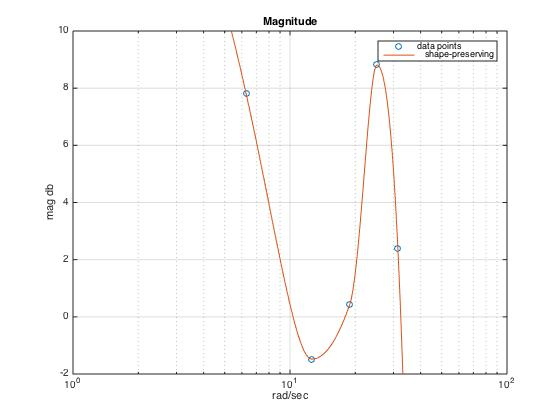
\includegraphics[scale=0.6]{experimentalBodeMag}
			\caption{Experimental Bode Plot Magnitude}
		\end{figure}
		\begin{figure}[H]
			\centering
			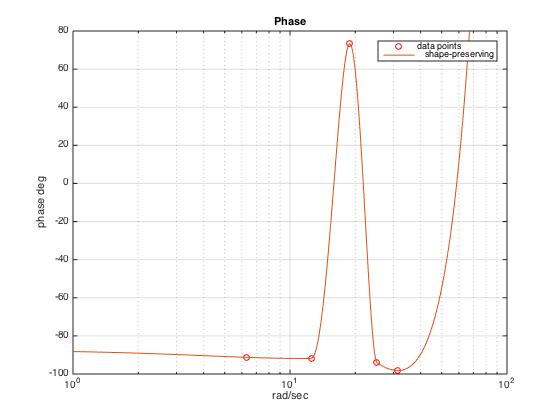
\includegraphics[scale=0.6]{experimentalBodePhase}
			\caption{Experimental Bode Plot Phase}
		\end{figure}
	\subsection{Solutions Part II}
		A final aspect pertaining to the frequency response was to use the least squares method to determine the unknown coefficients from the equations of motion. Adding the middle disc to the TDS system introduces new unknown parameters as shown in the below equations.
		\begin{align}
			J_1\dot{\omega_1} &+ c_1\omega_1 + k\beta - bu = 0 \\
			J_2\dot{\omega_2} &+ c_2\omega_2 -k\beta = 0 \\
			\dot{\beta} &= \omega_1 - \omega_2
		\end{align}
		The least squares equation $x =A \setminus b$ can again be used to solve for the unknowns in the $x$ vector. All other variables can be calculated from the equations in section \ref{sec:eq}.
		\begin{equation}
			\begin{bmatrix}
				c_1 \\
				k \\
				b \\
			\end{bmatrix}
			=
			\begin{bmatrix}
				\omega_1 & (\Theta_1 - \Theta_2) & -u \\
			\end{bmatrix}
			\setminus
			\begin{bmatrix}
				-J_1\dot{w_1}
			\end{bmatrix}
		\end{equation}\\
		\begin{equation}
			\begin{bmatrix}
				c_2 \\
				k
			\end{bmatrix}
			=
			\begin{bmatrix}
				w_2 & (\Theta_2 - \Theta_1) \\
			\end{bmatrix}
			\setminus
			\begin{bmatrix}
				-J_2\dot{w_2}
			\end{bmatrix}
		\end{equation}
		For the frequency $2\pi \mbox{ rad/sec}$ the calculated values are:
		\begin{align*}
			c_1 &= 0.00022632 \\
			c_2 &= 0.00010809 \\
			k &= 0.0117 \\
			b &= 0.0052 \\
		\end{align*}
		These values deviate from the calculated values using alternative methods but this could be due to noise in the experimental data or other unknowns.

\end{document}